\section{Results}

\subsection{Knowledge Graph Inspection and ABox Visualisation}

To verify the structural integrity of the constructed knowledge graph, the rich KG variant was loaded into GraphDB and inspected both visually and through SPARQL queries.

\subsubsection{ABox Visualisation}

\begin{figure}[H]
    \centering
    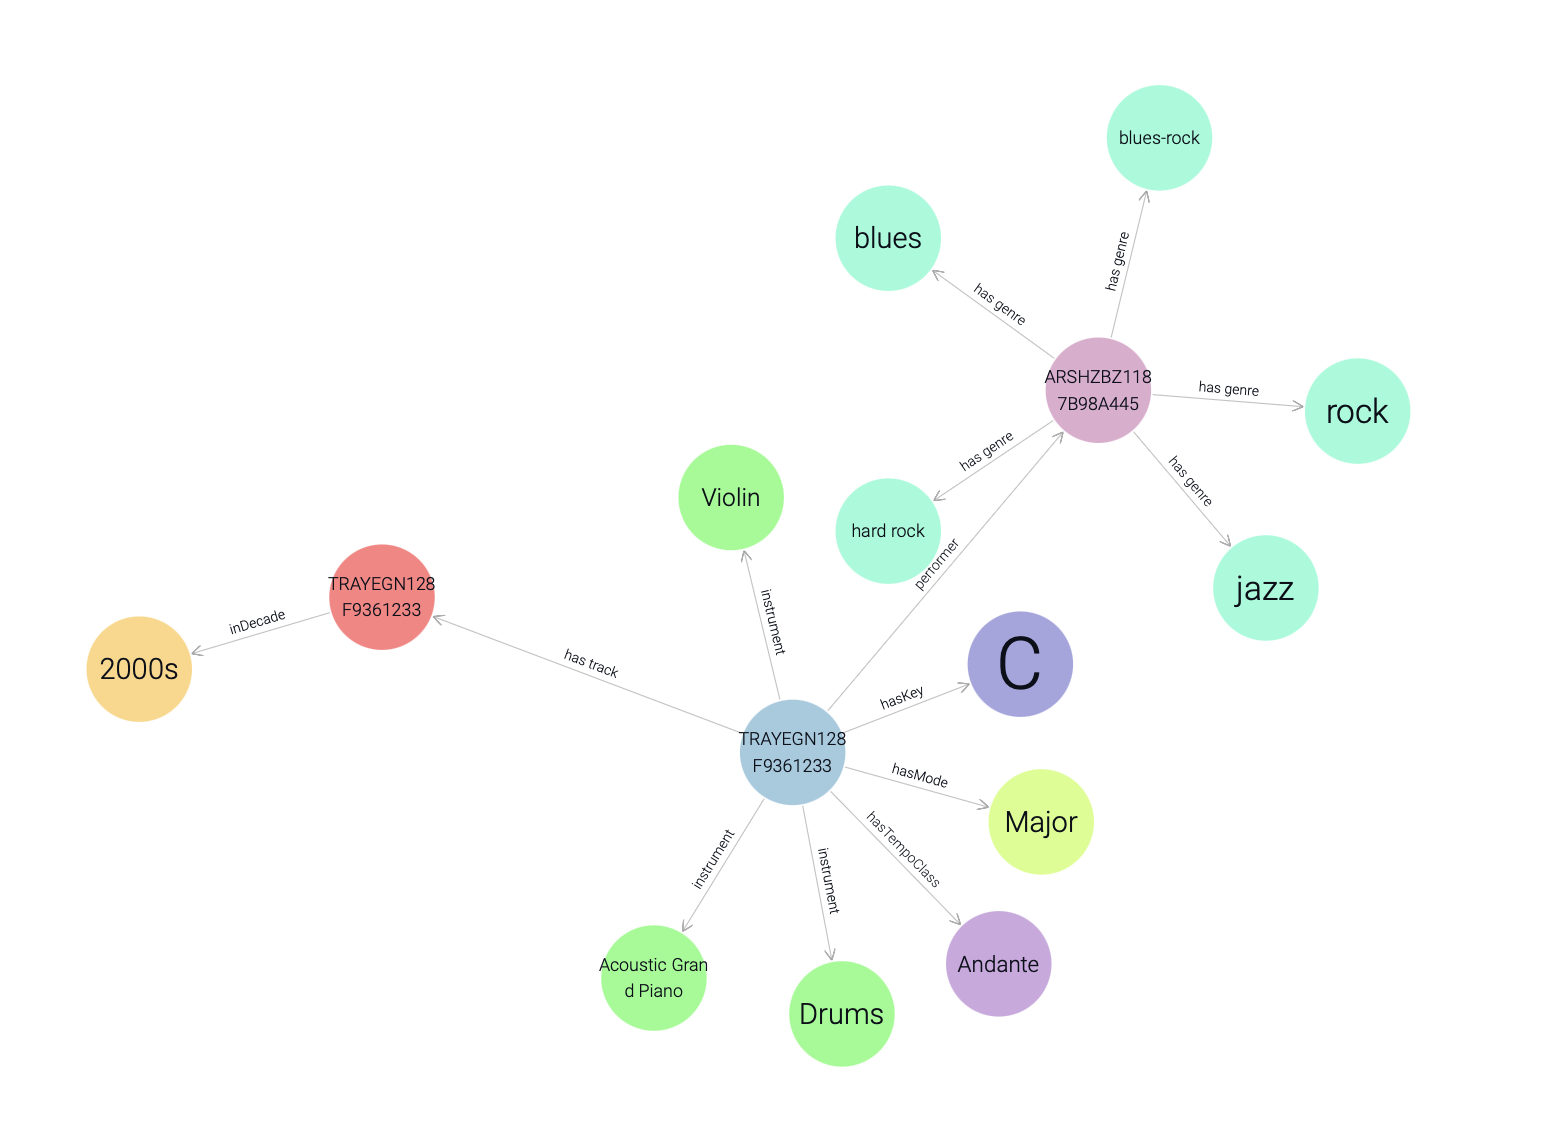
\includegraphics[width=0.75\linewidth]{sec/graph_DB/graph.png}
    \caption{GraphDB visual graph: ABox neighbourhood of a representative track instance (TRAYEGN128F9361233)}
    \label{fig:graph_vis}
\end{figure}

Figure~\ref{fig:graph_vis} shows the ABox neighbourhood of a representative track, \textit{When She Dances} (TRAYEGN128F9361233), as rendered by GraphDB's visual graph explorer. The central \texttt{mo:Performance} node fans out via \texttt{hasKey}, \texttt{hasMode}, and \texttt{hasTempoClass} edges (C, Major, Andante), three \texttt{mo:instrument} nodes (Violin, Acoustic Grand Piano, Drums), and a \texttt{performer} edge to artist Joe Bonamassa, which in turn links to five genre nodes. A \texttt{hasTrack} edge points to the \texttt{mrc:MSDTrack} node carrying the \texttt{mrc:inDecade} relation to the 2000s decade.

Inspecting the track node's properties (Figures~\ref{fig:1}--\ref{fig:3} in the Appendix) confirmed that all eleven jSymbolic audio features and bibliographic metadata are correctly stored on the \texttt{mrc:MSDTrack} instance, verifying that the builder pipeline fully populated both acoustic and descriptive dimensions.

Because, the visual explorer renders only named IRI nodes by default, so the \texttt{mrc:GenreAssociation} blank nodes carrying genre weights are not visible in Figure~\ref{fig:graph_vis}, and their presence was confirmed via a dedicated SPARQL query:

\begin{verbatim}
ASK { ?a mrc:hasGenreAssoc ?assoc .
      ?assoc mrc:weight ?w }
\end{verbatim}

which returned \texttt{true}. A subsequent \texttt{SELECT} query over the same artist retrieved five genre associations with descending weights: blues (1.0), blues-rock (0.6), hard rock (0.51), jazz (0.44), and rock (0.3). These weights reflect the proportional genre affinity of the artist as derived from the MSD tag data, and are stored as \texttt{xsd:double} literals on the intermediate blank node.


\subsubsection{Knowledge Graph Statistics and SPARQL Inspection}

The enriched knowledge graph contains 19,322,668 triples in total, and the node type histogram confirms the expected entity composition: 285,037 listeners, 7,013 tracks, 7,013 performances, 3,668 artists, 1,046 genres, 173 instruments, 14 decades, 12 keys, and 17 tempo classes. Hierarchy traversal queries confirmed that all genre and instrument nodes were correctly linked to their Wikidata super-classes, with genre nodes tracing through music genre and musical concept, and instrument nodes through their specific instrument families up to musical instrument. Similarly, the decade chain query confirmed that all decade nodes from the 1950s to the 2020s were correctly linked via temporal predecessor/successor relations and assigned to their parent century (20th or 21st).

Genre ranking queries revealed that rock is the most frequently occurring genre by artist count (2,117 artists), followed by popular music and pop (1,062 each) and electronic (1,037). When ranked by aggregated weight in the rich KG, the ordering shifts notably: hip-hop subgenres (hardcore hip hop, instrumental hip hop, jazz hip hop, etc.) rise to the top with a total weight of 2,405 across 385 artists, reflecting higher per-artist term weights despite fewer artists than rock, demonstrating how the weighted representation in the rich KG captures genre salience more faithfully than raw artist counts alone. 

\begin{figure}[H]
    \centering
    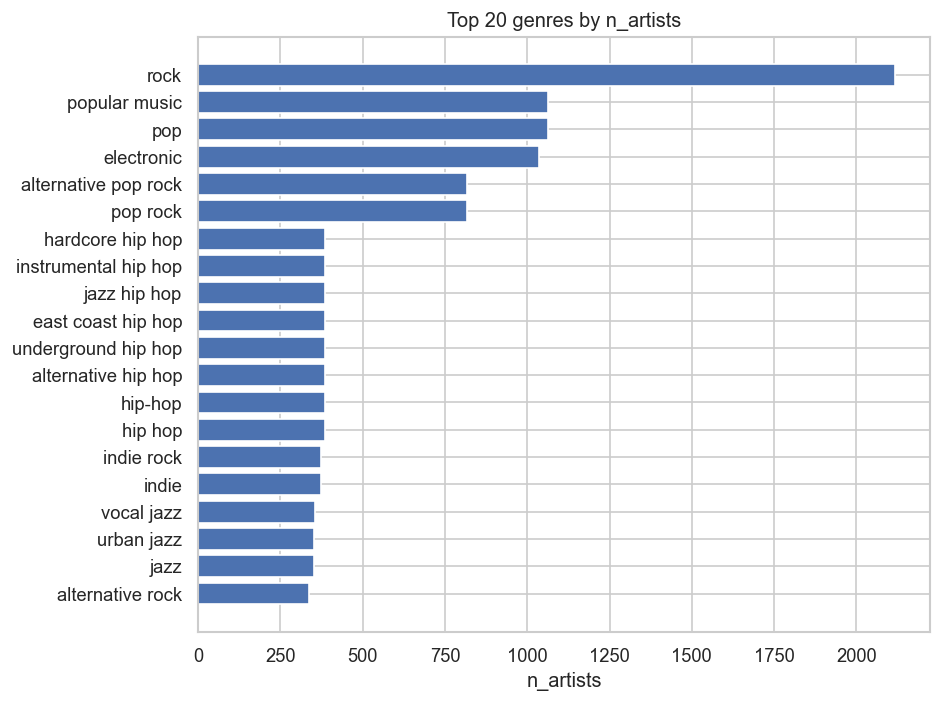
\includegraphics[width=0.75\linewidth]{sec/kg_plots/genres_simple.png}
    \caption{Top 20 genres by n\_artists (simple KG)}
    \label{fig:genres_simple}
\end{figure}

\begin{figure}[H]
    \centering
    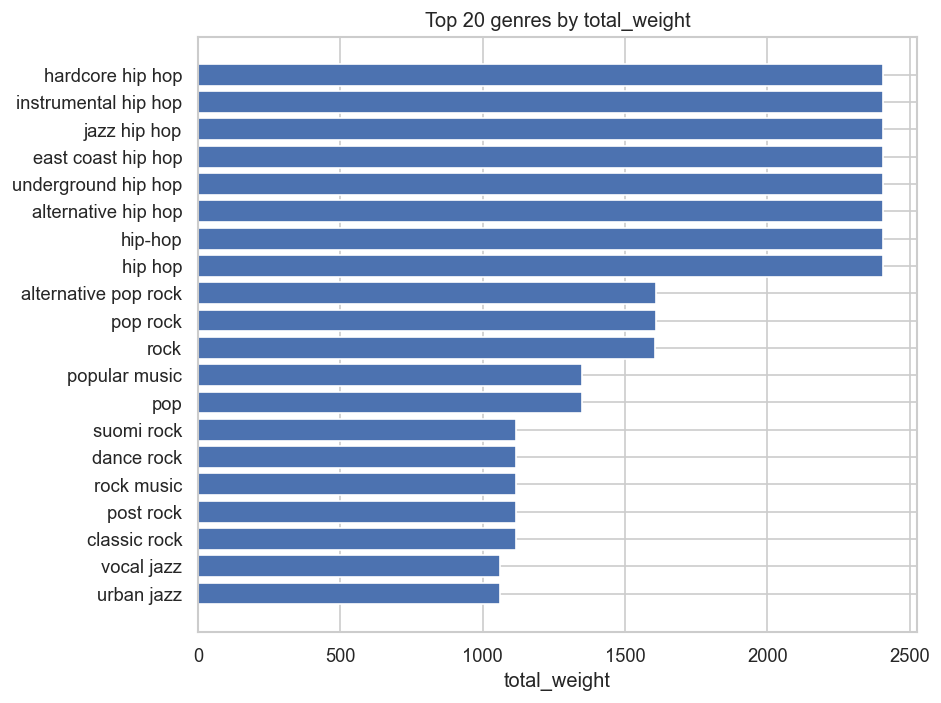
\includegraphics[width=0.75\linewidth]{sec/kg_plots/genres_rich.png}
    \caption{Top 20 genres by total\_weight (rich KG)}
    \label{fig:genres_rich}
\end{figure}

Key distribution queries on the rich KG, filtered to 
high-confidence detections ($\mathit{keyConfidence} \geq 0.8$), 
showed that C major is the most common key (211 tracks), 
followed by G (196) and D (150), being consistent with the 
prevalence of these keys in Western popular music.

\begin{figure}[H]
    \centering
    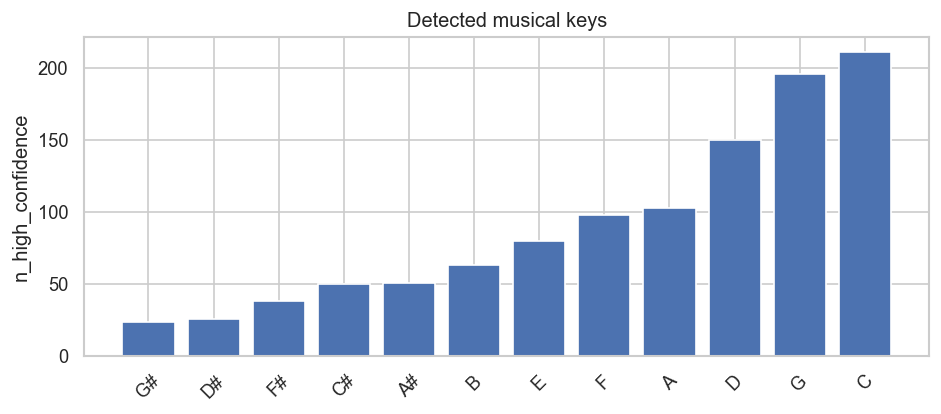
\includegraphics[width=0.75\linewidth]{sec/kg_plots/confident_keys_rich.png}
    \caption{Distribution of High-Confidence Musical Keys}
    \label{fig:confidence_keys}
\end{figure}

Lastly, through graph exploration we found out that the most listened-to track in the dataset was \textit{Secrets} by OneRepublic, played by 50,058 distinct users with a total of 197,579 plays, followed by \textit{You're The One} by Dwight Yoakam (42,810 listeners, 390,283 total plays, the highest total play count in the dataset).

Overall, the SPARQL inspection confirmed that the knowledge graph was correctly populated and structurally sound, with ontological alignments, temporal chains, and entity counts all matching the expected design. The genre ranking comparison between the two KG variants illustrated the added expressiveness of the weighted representation, while the key distribution and popularity queries provided initial insights into the musical and behavioural characteristics of the dataset.

\subsection{Autoencoder Reconstruction Results}

The autoencoder trained for the full 200 epochs, as the early stopping criterion - no improvement greater than 10-410\^{-4}
10-4 over 15 consecutive epochs — was never triggered, indicating that the loss continued to decrease, albeit slowly, throughout training. The MSE fell from 0.96 at epoch 0 to 0.62 at epoch 200, with the steepest descent in the first 75 epochs followed by a gradual flattening. The final reconstruction loss of 0.62 confirms that the 128-dimensional bottleneck retains sufficient information to approximately reconstruct the 1,526-dimensional input.



\subsection{Baseline Model Results}

The KNN collaborative filter sweep over the validation set selected $k = 6$ neighbours as optimal, balancing ranking quality against catalogue coverage. At $k = 6$ on the test set, KNN-CF achieved Recall@10 of 0.104, NDCG@10 of 0.106, Hit Rate@10 of 0.170, and MRR of 0.087, with a catalogue coverage of 91.5\% and a low popularity bias of 0.133, indicating that the model recommends diverse, non-mainstream items.

The most-popular baseline achieved a comparable Hit Rate@10 of 0.184 and slightly lower NDCG@10 of 0.098. Its catalogue coverage was although only 0.2\%, meaning it effectively recommends the same small set of globally popular tracks to every user. Its popularity bias score of 0.628 confirms this. The overall score (a composite metric) was 0.134 for popularity versus 0.420 for KNN-CF, largely driven by the coverage difference.

An XGBoost hybrid reranker was also evaluated at $K = 10$, yielding Recall@10 of 0.038, NDCG@10 of 0.044, and Hit Rate@10 of 0.072, substantially below KNN-CF. Its coverage (66.7\%) and low popularity bias (0.118) suggest it diversifies recommendations, but the retrieval bottleneck limits absolute ranking performance.

Together, the baselines establish that a simple collaborative filter already substantially outperforms popularity-based recommendation in ranking quality and catalogue diversity, setting a meaningful bar for the HGT model.